\chapter{Линейная фильтрация}

\section{Цель работы}
Изучить воздействие ФНЧ на тестовый сигнал с шумом.

\section{Постановка задачи}
Сгенерировать гармонический сигнал с шумом и синтезировать ФНЧ. Получить сигнал во временной и частотной областях до и после фильтрации. Сделать выводы о воздействии ФНЧ на спектр сигнала.

\section{Ход работы}
Линейный фильтр - динамическая система, применяющая некий линейный оператор ко входному сигналу для выделения или подавления определенных частот сигнала и других функций по обработке входного сигнала.
Фильтр Баттерворта - один из типов электронных фильтров. Фильтры этого класса отличаются от других методом проектирования. Фильтр Баттерворта проектируется так, чтобы его амплитудно-частотная характеристика
была максимально гладкой на частотах полосы пропускания.
В командном окне Matlab сгенерируем гармонический сигнал без шума
и с шумом, а также спектры сигнала с шумом и без шума. 

\subsection{Код Matlab}
\begin{lstlisting}
x = 0:0.01:4*pi;
f=100*(0:255)/512;
figure
noise=rand(size(x));
y = sin(2*pi*x);
y_noisy = y+0.3*noise;
%Построение сигнала без шума:
plot(x(1:200),y(1:200))
grid
%синтез ФНЧ Баттерворта
[B,A] = butter(16,0.99);
B=B./sum(B);
A=A./sum(A);
%обработка сигнала ФНЧ
figure
y_filtered = conv(y_noisy,[B,A]);
%Построение сигнала с шумом:
plot(x(1:200),y_filtered(1:200))
grid
figure
%Построение спектра сигнала с шумом
noisy_spectrum = fft(y_noisy,512);
norm_noisy_spectrum = noisy_spectrum.*conj(noisy_spectrum)/512;
%Построение нормирова спектра сигнала с шумом:
plot(f,norm_noisy_spectrum(1:256))
axis([0 max(f) 0 2])
grid
figure
%Спектр сигнала без шума
spectrum = fft(y_filtered,512);
norm_filtered_spectrum=spectrum.*conj(spectrum)/512;
%Построение нормированого спектра сигнала без шума:
plot(f,norm_filtered_spectrum(1:256))
axis([0 max(f) 0 2])
grid

\end{lstlisting}

\begin{figure}[H]
   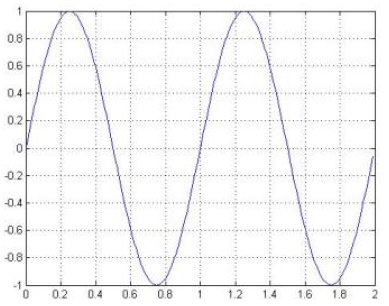
\includegraphics[scale=0.7]{lab6/1.png}
   \caption{Сигнал без шума}
\end{figure}

\begin{figure}[H]
   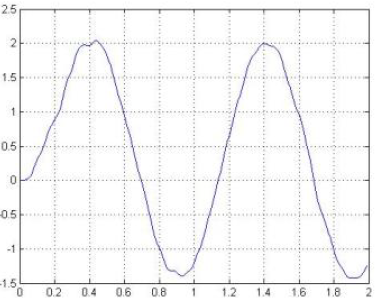
\includegraphics[scale=0.7]{lab6/2.png}
   \caption{Сигнал с шумом}
\end{figure}

\begin{figure}[H]
   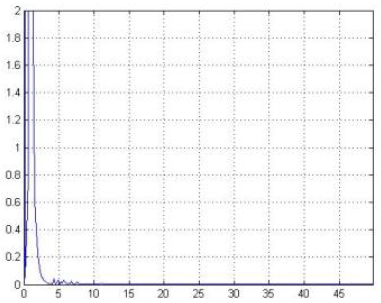
\includegraphics[scale=0.7]{lab6/3.png}
   \caption{Спектр сигнала без шума}
\end{figure}

\begin{figure}[H]
   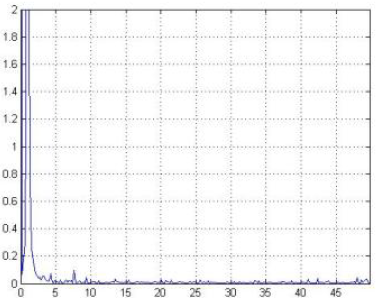
\includegraphics[scale=0.7]{lab6/4.png}
   \caption{Спектр сигнала с шумом}
\end{figure}

\subsection{Simulink}
Для создания модели в Simulink
используем блок Discrete FIR Filter раздела Discrete главной библиотеки и
блок Digital Filter design из Signal Processing Blockset/Filtering/Filter Designs.

\begin{figure}[H]
   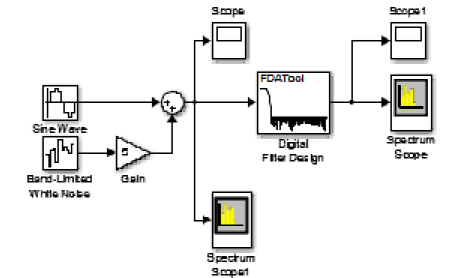
\includegraphics[scale=0.7]{lab6/5.png}
   \caption{Схема модели}
\end{figure}

\begin{figure}[H]
   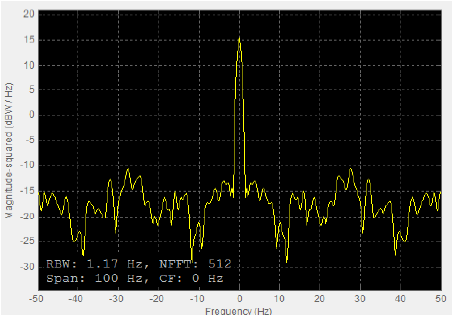
\includegraphics[scale=0.7]{lab6/6.png}
   \caption{Спектр до фильтрации}
\end{figure}

\begin{figure}[H]
   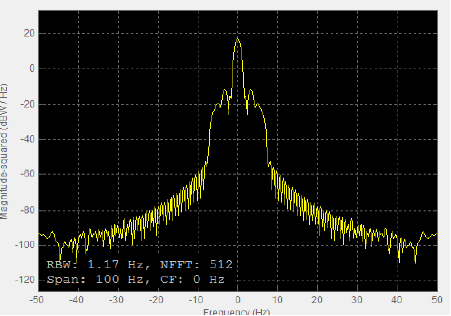
\includegraphics[scale=0.7]{lab6/7.png}
   \caption{Спектр после фильтрации}
\end{figure}
\begin{figure}[H]
   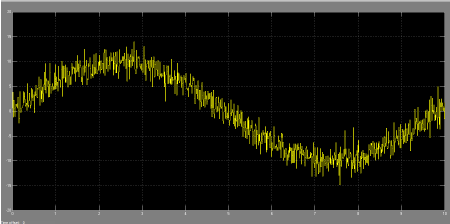
\includegraphics[scale=0.7]{lab6/8.png}
   \caption{Сигнал без шума}
\end{figure}

\begin{figure}[H]
   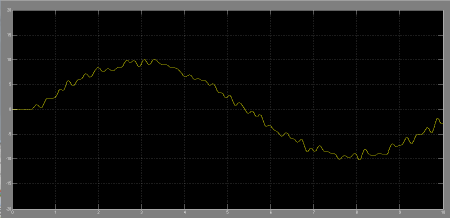
\includegraphics[scale=0.7]{lab6/9.png}
   \caption{Сигнал с шумом}
\end{figure}

\section{Вывод}

Фильтр нижних частот - вид фильтра, пропускающий частотный спектр сигнала ниже некоторой частоты (частоты среза), и подавляющий частоты сигнала выше этой частоты. Степень подавления каждой частоты зависит от
вида и порядка фильтра. Идеальный ФНЧ полностью подавляет все частоты входного сигнала выше частоты среза и пропускает без изменений все частоты ниже частоты среза.

В лабораторной работе мы произвели удаление шума линейным фильтром. Однако важно понимать, что линейные фильтры способны удалять только шум с частотой, отличающейся от частоты сигнала.